% Author @ Huyen Tran, DONE

%\subsection{Edmonds-Karp Algorithm}
\label{ek algo}

The \textbf{Edmonds-Karp algorithm}, developed by Jack Edmonds and Richard Karp in 1972, is an implementation of the Ford-Fulkerson method for computing the maximum flow in a flow network by using \textbf{breadth-first search (BFS)} to find the shortest augmenting paths in terms of edge count. \cite{edmonds_karp_1972}

\subsubsection*{Algorithm Overview}
The Edmonds-Karp algorithm operates in polynomial time and is based on the principle of finding the maximum flow in a flow network by augmenting flows along shortest paths. The process begins by initializing the flow at zero and constructing an initial feasible solution in the residual network. It then iteratively increases the flow by finding augmenting paths—shortest paths from the source to the sink in terms of edge count in the residual network—until no more augmenting paths exist, indicating an optimal solution.

\noindent In each iteration, the algorithm identifies the shortest augmenting path using BFS and adjusts the flow along this path by its minimum residual capacity. This approach ensures that each augmentation moves the flow closer to the maximum flow while maintaining a feasible flow throughout its execution. By using BFS to select augmenting paths, the Edmonds-Karp algorithm achieves a more efficient and practical implementation of the Ford-Fulkerson method, widely adopted for solving maximum flow problems in various fields.

\noindent The algorithm would take a graph instance \( G = (d, n, m, E) \), with parameters:
        \begin{itemize}
            \item \( d \): The degree of vertices in the matching,
            \item \( n \): The number of vertices on each side of the bipartite graph,
            \item \( m \): The number of edges, and
            \item \( E \): The set of edges connecting left and right vertex sets.
        \end{itemize}
        
\paragraph{Example:}
Below is an example bipartite graph with sets \( U = \{ u_1, u_2, u_3 \} \) and \( V = \{ v_1, v_2, v_3 \} \). The maximum matching is highlighted in red.

\begin{figure}[h!]
\centering
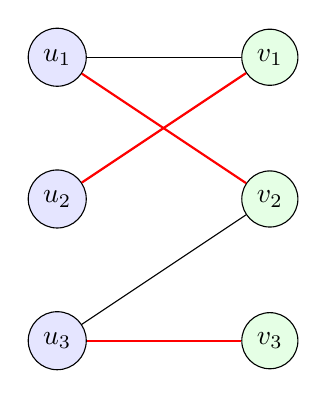
\begin{tikzpicture}[scale=0.9, every node/.style={circle, draw, minimum size=0.4cm}]
    % Nodes in U
    \node[fill=blue!10] (u1) at (0,2) {$u_1$};
    \node[fill=blue!10] (u2) at (0,0) {$u_2$};
    \node[fill=blue!10] (u3) at (0,-2) {$u_3$};
    
    % Nodes in V
    \node[fill=green!10] (v1) at (3,2) {$v_1$};
    \node[fill=green!10] (v2) at (3,0) {$v_2$};
    \node[fill=green!10] (v3) at (3,-2) {$v_3$};
    
    % Edges (Non-matching in black)
    \draw (u1) -- (v1);
    \draw (u1) -- (v2);
    \draw (u2) -- (v1);
    \draw (u3) -- (v2);
    \draw (u3) -- (v3);
    
    % Matching edges in red
    \draw[thick, red] (u2) -- (v1);
    \draw[thick, red] (u1) -- (v2);
    \draw[thick, red] (u3) -- (v3);
\end{tikzpicture}
\caption{A solved instance of the Maximum Matching Problem with $d = 2$, $|V| = 3$, $|E| = 5$. The black lines show the edges of $E$. The three edges highlighted in red are a maximum matching $M = \{ (u_1, v_2), (u_2, v_1), (u_3, v_3) \} $ of $G$.}
\label{fig:ex_bipartite_graph}
\end{figure}

\noindent Given the graph \( G = \{2, 3, 5, ((1,1), (1,2), (2,1), (3,2), (3,3)) \} \) as Figure \ref{fig:ex_bipartite_graph}, we can trace the Edmonds-Karp algorithm as follows:

\textbf{Initialization:} The residual graph is constructed with a source node \( s \) and sink node \( t \). Capacities are assigned such that:
\begin{itemize}
    \item \( c(s, u_i) = 1 \) for all \( u_i \in U \),
    \item \( c(v_j, t) = 1 \) for all \( v_j \in V \),
    \item \( c(u_i, v_j) = 1 \) for all \( (u_i, v_j) \in E \).
\end{itemize}
\par Initially, all flows \( f(u, v) \) are set to zero, and the residual capacities are equal to the original capacities.\\

\textbf{First Augmenting Path:} Using BFS, the algorithm identifies the first augmenting path:
$s \to u_1 \to v_1 \to t$.
\par The residual capacity of this path is: $c_f(p_1) = \min(c_f(s, u_1), c_f(u_1, v_1), c_f(v_1, t)) = \min(1, 1, 1) = 1.$
\par Flow Update:$f(s, u_1) = 1, \quad f(u_1, v_1) = 1, \quad f(v_1, t) = 1$.
\par Forward edges' residual capacities: $c_f(s, u_1) = 0, \quad c_f(u_1, v_1) = 0, \quad c_f(v_1, t) = 0.$
\par Reverse edges' capacities: $c_f(u_1, s) = 1, \quad c_f(v_1, u_1) = 1, \quad c_f(t, v_1) = 1.$\\

\textbf{Second Augmenting Path:} BFS finds another augmenting path: $s \to u_2 \to v_2 \to t.$
\par The residual capacity of this path is: $c_f(p_2) = \min(c_f(s, u_2), c_f(u_2, v_2), c_f(v_2, t)) = \min(1, 1, 1) = 1.$
\par Flow Update: $f(s, u_2) = 1, \quad f(u_2, v_2) = 1, \quad f(v_2, t) = 1.$
\par Forward edges' residual capacities: $c_f(s, u_2) = 0, \quad c_f(u_2, v_2) = 0, \quad c_f(v_2, t) = 0.$
\par Reverse edges' capacities: $c_f(u_2, s) = 1, \quad c_f(v_2, u_2) = 1, \quad c_f(t, v_2) = 1.$\\

\textbf{Third Augmenting Path:} BFS identifies another path: $s \to u_3 \to v_3 \to t.$
\par The residual capacity of this path is: $c_f(p_3) = \min(c_f(s, u_3), c_f(u_3, v_3), c_f(v_3, t)) = \min(1, 1, 1) = 1.$
\par Flow Update: $f(s, u_3) = 1, \quad f(u_3, v_3) = 1, \quad f(v_3, t) = 1.$
\par Forward edges' residual capacities: $c_f(s, u_3) = 0, \quad c_f(u_3, v_3) = 0, \quad c_f(v_3, t) = 0.$
\par Reverse edges' capacities: $c_f(u_3, s) = 1, \quad c_f(v_3, u_3) = 1, \quad c_f(t, v_3) = 1.$\\

\textbf{Termination:} BFS is unable to find any additional augmenting paths, as no path from $s$ to $t$ with positive residual capacity exists. The algorithm terminates.

\textbf{Extracting the Matching:} The matching is extracted by identifying edges $(u_i, v_j)$ in the residual graph where reverse edges \( (v_j, u_i) \) have positive capacity. The resulting maximum matching is:
\[
M = \{ (u_1, v_2), (u_2, v_1), (u_3, v_3) \}.
\]
\par This matching corresponds to the edges highlighted in red in the original graph.


\subsubsection*{Performance and Time Complexity}

The Edmonds-Karp algorithm has a time complexity of \(\mathcal{O}(VE^2)\), which is polynomial in the number of vertices \( V \) and edges \( E \) of the graph. The analysis of this complexity relies on two key theoretical results, a lemma and a theorem, which bound the number of augmenting paths and explain how the structure of the residual network changes over time.

\begin{lemma}
If the Edmonds-Karp algorithm is run on a flow network \( G = (V, E) \) with source \( s \) and sink \( t \), then for all vertices \( v \in V \setminus \{s, t\} \), the shortest-path distance \( \delta_f(s, v) \) in the residual network \( G_f \) increases monotonically with each flow augmentation.
\end{lemma}
This lemma states that in the Edmonds-Karp algorithm, the shortest-path distance \( \delta_f(s, v) \) from the source \( s \) to any vertex \( v \) in the residual network \( G_f \) either increases or remains constant with each flow augmentation. This property ensures that distances in the residual network do not decrease, helping to limit the number of augmenting paths that can be selected over the course of the algorithm.

\begin{theorem}
    If the Edmonds-Karp algorithm is run on a flow network \( G = (V, E) \) with source \( s \) and sink \( t \), then the total number of flow augmentations performed by the algorithm is \( O(VE) \).
\end{theorem}
This theorem states that the total number of augmenting paths required by the Edmonds-Karp algorithm to reach the maximum flow is \(\mathcal{O}(VE)\). Each edge in the residual network can become critical (limiting the residual capacity of a path) at most \(\mathcal{O}(V)\) times. This bound prevents the algorithm from cycling inefficiently through paths, as each critical edge reappearance increases the shortest-path distance of involved vertices, further limiting augmenting path frequency.

Together, these results guarantee that the Edmonds-Karp algorithm performs only a limited, polynomial number of augmentations. Each BFS search to find an augmenting path takes \( \mathcal{O}(E) \) time, leading to an overall complexity of \( \mathcal{O}(VE^2) \).\\

\noindent Further details and implementation of this algorithm is discussed in Section \ref{ekImplement}
